\let\negmedspace\undefined
\let\negthickspace\undefined
\documentclass[journal,12pt,onecolumn]{IEEEtran}
\usepackage{cite}
\usepackage{amsmath,amssymb,amsfonts,amsthm}
\usepackage{algorithmic}
\usepackage{graphicx}
\graphicspath{{./figs/}}
\usepackage{textcomp}
\usepackage{xcolor}
\usepackage{txfonts}
\usepackage{listings}
\usepackage{enumitem}
\usepackage{mathtools}
\usepackage{gensymb}
\usepackage{comment}
\usepackage{caption}
\usepackage[breaklinks=true]{hyperref}
\usepackage{tkz-euclide} 
\usepackage{listings}
\usepackage{gvv}                                        
%\def\inputGnumericTable{}                                 
\usepackage[latin1]{inputenc}     
\usepackage{xparse}
\usepackage{color}                                            
\usepackage{array}
\usepackage{longtable}                                       
\usepackage{calc}                                             
\usepackage{multirow}
\usepackage{multicol}
\usepackage{hhline}                                           
\usepackage{ifthen}                                           
\usepackage{lscape}
\usepackage{tabularx}
\usepackage{array}
\usepackage{float}
\newtheorem{theorem}{Theorem}[section]
\newtheorem{problem}{Problem}
\newtheorem{proposition}{Proposition}[section]
\newtheorem{lemma}{Lemma}[section]
\newtheorem{corollary}[theorem]{Corollary}
\newtheorem{example}{Example}[section]
\newtheorem{definition}[problem]{Definition}
\newcommand{\BEQA}{\begin{eqnarray}}
\newcommand{\EEQA}{\end{eqnarray}}
\newcommand{\define}{\stackrel{\triangle}{=}}
\theoremstyle{remark}
\newtheorem{rem}{Remark}

\begin{document}
\title{1.6.6}
\author{ee25btech11056 - Suraj.N}
\maketitle
\renewcommand{\thefigure}{\theenumi}
\renewcommand{\thetable}{\theenumi}

In each of the following, find the value of $k$ for which the points are collinear:
\begin{enumerate}
\item $\brak{7,-2},\ \brak{5,1},\ \brak{3,k}$
\item $\brak{8,1},\ \brak{k,-4},\ \brak{2,-5}$
\end{enumerate}

\textbf{Solution:} Three points $A, B, C$ are collinear iff the collinearity matrix
\begin{align*}
M=\myvec{ \vec{B}-\vec{A} & \vec{C}-\vec{A} }^\top
\end{align*}
has $rank\brak{M}=1$.

\textbf{(a)} 

\begin{align*}
\myvec{ \vec{B}-\vec{A} & \vec{C}-\vec{A} }^\top = \myvec{-2 & 3\\ -4 & k+2}
\end{align*}

\begin{align*}
\myvec{-2 & 3\\ -4 & k+2}
&\xleftrightarrow{R_2 = R_2 - 2R_1}
\myvec{-2 & 3\\ 0 & k-4}
\end{align*}

For collinearity, $rank\brak{M}=1 \iff k-4=0 \implies \boxed{k=4}$.

\textbf{(b)} 

\begin{align*}
\myvec{ \vec{B}-\vec{A} & \vec{C}-\vec{A} }^\top = \myvec{k-8 & -5\\ -6 & -6}
\end{align*}

\begin{align*}
\myvec{k-8 & -5\\ -6 & -6}
&\xleftrightarrow{R_2 = (k-8)R_2 + 6R_1}
\myvec{k-8 & -5\\[2pt] 0 & 18-6k}
\end{align*}
For collinearity, $rank\brak{M}=1 \iff 18-6k=0 \implies \boxed{k=3}$.

\pagebreak

\begin{figure}[h!]
  \centering
  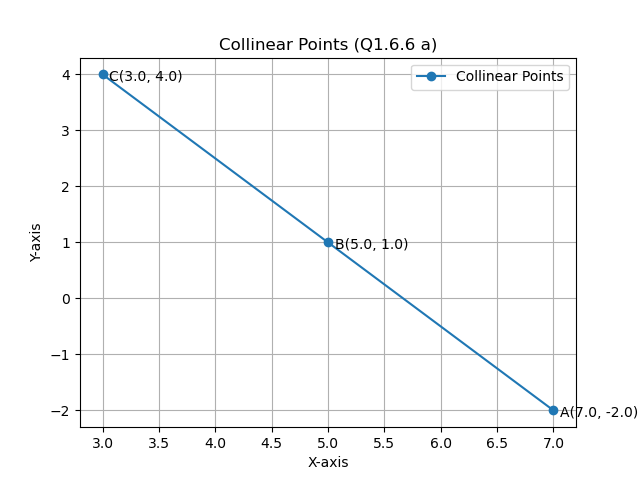
\includegraphics[width=0.5\columnwidth]{figs/fig_a.png} 
   \caption*{Fig 1 : Line through the given points}
  \label{Fig1}
\end{figure}

\begin{figure}[h!]
  \centering
  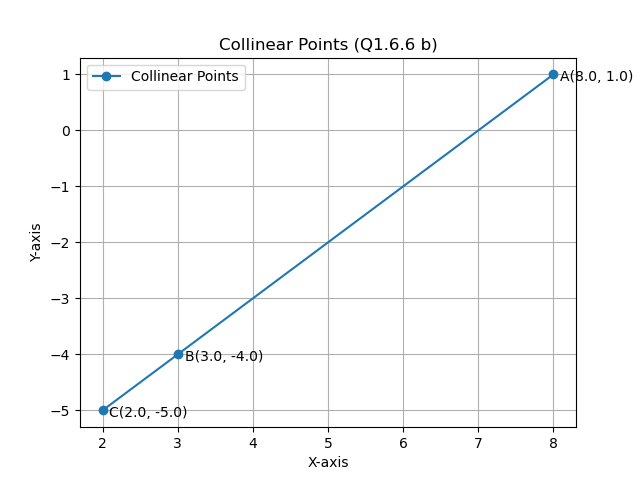
\includegraphics[width=0.5\columnwidth]{figs/fig_b.png} 
   \caption*{Fig 2 : Line through the given points}
  \label{Fig2}
\end{figure}


\end{document}
